\appendix
\section{Appendix}
\subsection{Variables of the HMDP topic model}
\label{hmdpvars}
As adopted from Kling \cite{DBLP:phd/dnb/Kling16}.
\begin{table}[H]
\caption{Variables of the hierarchical multi-Dirichlet process topic model \cite{DBLP:phd/dnb/Kling16}.}
\begin{tabular}{ll}
\hline
$M$ & Number of documents \\
$N_m$ & Number of words in document $m$ \\
$F$ & Number of context spaces \\
$C_f$ & Number of context clusters for context space $f$ \\
$A_f$ & Number of context groups with common parents in context space $f$ \\
$\beta_0$ & Concentration parameter of the topic prior \\
$H$ & Space of all possible topic multinomials, with Dirichlet prior $\beta_0$ \\
$G_0$ & Global measure on the topic space (includes topics and their weight) \\
$G_{fj}^c$ & Measure on the topic space for cluster $j$ of context space $f$ \\
$G_m^d$ & Document-specific measure on the topic space \\
$\gamma$ & Scaling parameter of the global Dirichlet process (DP) \\
$\alpha_0$ & Scaling parameter for the context cluster DPs \\
$\alpha_1$ & Scaling parameter for the document MDPs \\
$\phi_{mn}$ & Topic drawn for $w_{mn}$ \\
$w_{mn}$ & Word $n$ for document $m$ \\
$g_{mf}$ & Context group of document $m$ in context space $f$ \\
$\zeta$ & Mixing weights for the context spaces \\
$\eta_{fi}$ & Mixing weights for the group $i$ in context space $f$ \\
$\varepsilon$ & Concentration parameter of the Dirichlet prior on $\zeta$ \\
$\delta_f$ & Concentration parameter of the Dirichlet prior on $\eta$ in context space $f$
\end{tabular}
\end{table}

\newpage
\subsection{Annotations of the YNACC subset annotated by experts}
\label{ynacclabel}
\begin{table}[H]
\caption{The annotations for each comment in the YNACC subset annotated by experts as outlined in \cite{napoles2017ynacc} and available under \url{https://github.com/cnap/ynacc}.}
\begin{tabular}{ll}
\hline
sdid & Subdialog id, identifies the comment thread of a comment.\\
commentindex & Position of the comment in the thread.$m$ \\
headline & Headline of the article the comment was issued under.\\
url & URL of the article. \\
guid & Encrypted user id. \\
commentid & Comment id.\\
timestamp & Timestamp of when the comment was issued. \\
thumbs-up & No. of upvotes. \\
thumbs-down & No. of downvotes.\\
text & Comment text. \\
parentid & ID of the first comment in the subdialogue. \\
constructiveclass & Whether a comment was constructive or not. \\
\texttt{sd\_agreement} & (Dis-) agreement throughout the subdialogue. \\
\texttt{sd\_type} & Type of converstation in the subdialogue. \\
sentiment & Sentiment label of the comment. \\
tone & Tone of the comment. \\
commentagreement & (Dis-) agreement of the comment. \\
topic & Whether the comment was on- or off-topic \\
intendedaudience & Broadcast or reply. \\
persuasiveness & Whether the comment was persuasive or not.
\end{tabular}
\end{table}

\newpage

\subsection{Proof of claim in Section 4}
\begin{proof}
\label{partitionproof}
Let $M,K >0$ and $N = M+K$.
\begin{align}
\binom{N}{2} &= \binom{M+K}{2} = \frac{1}{2}(M+K)(M+K-1) \\
&= \frac{1}{2}(M^2+K^2+2MK-M-K) \\
&> \frac{1}{2}(M^2+K^2-M-K) = \frac{1}{2}\left(M(M-1)+K(K-1)\right) \\
&= \binom{M}{2}+\binom{K}{2}
\end{align}
\end{proof}

\subsection{Proof of claim in Section 4.3}
\begin{proof}
\label{labelproof}
Let $X$ be a discrete random variable denoting a draw of a word from the set of words $W$, the sample space, denoting the words representing topic $t$. Then $X \sim \phi$ is distributed according to the multinomial distribution $\phi$ which denotes the topic-word distribution of the topic model. Let $L$ be the set of labels and $x \in L$ be a label which solely has the largest intersection $x \cap W$ and thus $x = \argmax_{l \in L} |l \cap W|$. Let $y \in L$ be a label with $|x \cap W| > |y \cap W| \Leftrightarrow |x \cap W| = |y \cap W| + a$ with $a \geq 1$. Suppose $y$ was chosen as a label, then:
\begin{equation}
y = \argmax_{l \in L} \left( |l \cap W| + \sum_{w \in (l \cap W)} P(w|\phi) \right)
\end{equation}
and thus:
\begin{align}
|y \cap W| + \sum_{w \in (y \cap W)} P(w|\phi) &\geq |x \cap W| + \sum_{w \in (x \cap W)} P(w|\phi) \\
\Leftrightarrow y \cap W| + \sum_{w \in (y \cap W)} P(w|\phi) &\geq a + |y \cap W| + \sum_{w \in (x \cap W)} P(w|\phi) \\
\Leftrightarrow \sum_{w \in (y \cap W)} P(w|\phi) &\geq a + \sum_{w \in (x \cap W)} P(w|\phi) \\
\end{align}
However, as $a > 1 \land 1 \geq \sum_{w \in (x \cap W)} P(w|\phi) > 0$ \footnote{It is strictly greater 0 as otherwise the n-gram x could not have occured under the model with topic-word distribution $\phi$.} this would be equivalent to:
\begin{equation}
\sum_{w \in (y \cap W)} P(w|\phi) > 1
\end{equation} which is trivially false as $\sum_{x \in W} P(X=x) = P(W) = 1$. Therefore it holds:
\begin{equation}
|x \cap W| + \sum_{w \in (x \cap W)} P(w|\phi) > |y \cap W| + \sum_{w \in (y \cap W)} P(w|\phi)
\end{equation}
Thus, $y$ can not have been the chosen label if it fulfills the equation. Instead, $x$ would be the chosen label and every label which fulfills the equation \begin{equation}
x = \argmax_{l \in L} \left( |l \cap W| + \sum_{w \in (l \cap W)} P(w|\phi) \right)
\end{equation} fulfills 
\begin{equation}x = \argmax_{l \in L} |l \cap W|.
\end{equation} Therefore, the labels found by the outlined algorithm fulfill said equation.
\end{proof}

\subsection{Topic evolution over time}
\label{topic_evo}
\begin{figure}[H]%
\centering
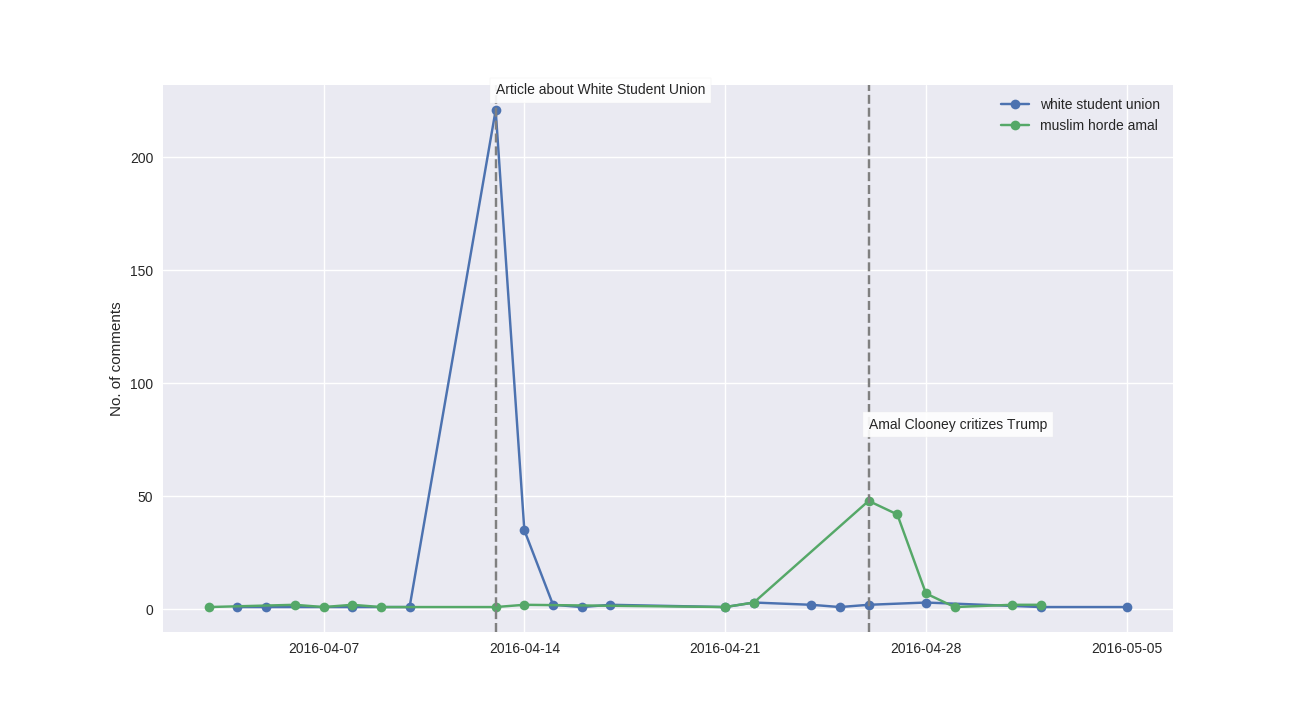
\includegraphics[width=\textwidth]{img/topic_evolution.png}%
\caption{Evolution of two topics of dataset \#3 over time with notable events marked.}
\end{figure}
This figure illustrates how the timely evolution of topics can be visualized. This is especially interesting, when there are multiple notable events and articles on a topic over time.